% Standalone draft of the experimental-evaluation part, 2026-08-12.
% Compile here: latexmk -pdf evaluation-draft.tex   (IEEEtran.cls is local).
% Intended fate: sections get merged into main.tex per
% docs/superpowers/specs/paper-edits-required-2026-08-12.md; equation and
% figure numbering will be reconciled at merge time. Citations reuse
% reference.bib keys. Every number is traceable to a CSV in Image/.

\documentclass[a4paper,conference]{IEEEtran}
\usepackage{cite}
\usepackage{amsmath,amssymb,amsfonts}
\usepackage{graphicx}
\usepackage{booktabs}
\usepackage{url}

\begin{document}

\title{Experimental Evaluation of Dynamic-Fee Hooks\\ (draft section for the ICBC paper)}
\maketitle

\section{Experimental Evaluation}
\label{sec:evaluation-draft}

The framework's evaluation layer runs every fee policy and a family of
static baselines over identical replayed market histories and scores the
liquidity provider (LP) against simply holding the deposited tokens. This
section describes the simulated market, the two-flow trader model, the
experiment design, and the results.

\subsection{Simulated Market and Reproducibility}

The experiment is a factorial matrix; one \emph{cell} of it --- one
combination of fee policy, trading pair, day-window, and gas-price
scenario --- replays a \emph{window} of 1{,}440 one-minute Binance
candles from 2024 against a Uniswap~v4 pool holding a 20M~USDT basket,
split equally by value into a full-range position. The pool opens at the external market price of the first
candle; a mock Chainlink-compatible feed tracks each candle's close; the
first 60 candles execute but are excluded from measurement. Three pairs
are studied: ETH/SHIB and ETH/USDC (volatile) and USDC/USDT (stable,
with a synthetic unit feed for its second leg). Windows are stratified
by realized volatility into terciles --- 24 calm, 24 medium, and 24
stormy days per pair --- so market regimes are represented by design.

Every cell records the manifest of Eq.~(M9)\footnote{References of the
  form Eq.~(M$n$) point to equation $n$ of the \emph{main paper}
  (\texttt{main.tex}), not to this draft's own numbering; they become
  ordinary \texttt{\textbackslash ref}s at merge time. Here: Eq.~(M9) is
the run identity $E=\langle C_{\theta},D,P_0,L_0,W,S\rangle$.}: the
configured contract,
a hash of the full contract source tree, the initial price and
liquidity, a fingerprint of the window's own candles, and the RNG seed.
A rerun skips cells whose manifest matches, and any change to a
contract or input invalidates exactly the affected cells. Because every
swap executes in a real EVM (Foundry), gas is \emph{measured} rather
than assumed: a calibration run records each policy's median gas per
swap (76k for the static hook, 88--124k for the adaptive ones), and
these measured figures feed back into both traders' decisions below.
Fees follow v4 accounting exactly: they accrue to the position and do
not compound. As an end-to-end validity check, the LP's holdings are
reconstructed independently from pool state and from trader flows; the
two ledgers agree to a relative error of ${\sim}10^{-16}$ on every cell.

\subsection{Two-Flow Trader Model}

Following the standard microstructure framing, order flow is split into
an informed arbitrageur and uninformed users (UU).

\subsubsection{Arbitrageur}
With fee fraction $f$ and $\gamma=1-f$, the pool price may sit anywhere
inside the no-arbitrage band $[P\gamma,\,P/\gamma]$ around the external
price $P$. Once per candle, after the retail flow, the arbitrageur moves
the pool to the nearest band edge if that trade is profitable
\emph{after gas}: with pool liquidity $L$, sqrt-price $s$ and target
$t$, the closed-form profit
\begin{equation}
  \Pi^{*}_{0\to1}=\frac{L(s-t)^{2}}{s},\qquad
  \Pi^{*}_{1\to0}=\frac{L(t-s)^{2}}{\gamma s},
  \label{eq:arb-profit}
\end{equation}
must exceed $g\,p_{\mathrm{gas}}$, where $g$ is the policy's measured
median gas and $p_{\mathrm{gas}}$ the scenario's gas price (5, 20, or
80~gwei), valued at the ETH price series. For the size-dependent
\texttt{MEVChargeHook} the optimum is found by ternary search; profit is
unimodal in size. $\Pi^{*}$ is a decision quantity only: all reported
metrics are computed from the balance changes of executed swaps.

\subsubsection{Uninformed users}
UU behavior follows the acceptance model of our prior work
\cite{lebedeva2025dynamic}: a candidate trade evaluates the normalized
outcome ratio
\begin{equation}
  r=\frac{V_{\mathrm{out}}-V_{\mathrm{in}}-G}
  {V_{\mathrm{out}}+V_{\mathrm{in}}+G},
  \label{eq:uu-r}
\end{equation}
where $V_{\mathrm{in}}$ and $V_{\mathrm{out}}$ are the two legs valued
at external prices --- so fee \emph{and} slippage are inside $r$ --- and
$G$ is the trade's own gas. Execution is probabilistic,
\begin{equation}
  P_{\mathrm{exec}}=
  \begin{cases}
    1, & r\ge 0,\\
    e^{-\lambda|r|}, & r<0,
  \end{cases}
  \label{eq:uu-p}
\end{equation}
with a sensitivity calibration $\lambda=\ln 2/|r(30\,\mathrm{bps})|
\approx 461.4$: half of the willing flow declines at a 30~bps total
transaction cost. ($\lambda$ is a stated assumption and is varied in
  sensitivity analysis; at our trade sizes the uncalibrated
$e^{-|r|}$ is insensitive to any fee in the box.)

Each minute $c$, each direction independently draws one candidate trade
of size
\begin{equation}
  q(c)=\frac{v_0(c)}{2}\;e^{\sigma Z-\sigma^{2}/2},
  \qquad Z\sim\mathcal{N}(0,1),\ \ \sigma=1,
  \label{eq:uu-size}
\end{equation}
where $v_0(c)$ is the minute's potential demand
(Eq.~\eqref{eq:uu-demand} below), split equally between the two
directions. The lognormal multiplier is mean-preserving
($\mathbb{E}[e^{\sigma Z-\sigma^{2}/2}]=1$), so randomness produces
realistic heavy-tailed trade sizes without distorting the calibrated
volume; the trade then executes all-or-nothing with probability
$P_{\mathrm{exec}}$. Discreteness is essential: it displaces the pool
(giving the arbitrageur work), gives each trade a definite gas bill, and
keeps randomness reproducible --- all draws are pre-generated from a
recorded seed. One draw per direction per minute is the lumpiest reading
of the measured volume and is declared as a limitation.

\subsubsection{Demand calibration}
The \emph{shape} of retail demand is measured: with $\hat{s}(c)$ the
2024 intraday profile of the pair's constituent Binance markets
(geometric mean of the two legs' per-minute quote volume, normalized to
sum to one over an average day), the potential demand of minute $c$ is
\begin{equation}
  v_{0}(c)=\kappa\cdot \mathrm{basket}\cdot\hat{s}(c),
  \label{eq:uu-demand}
\end{equation}
so the single free parameter $\kappa$ is the pool's daily turnover in
baskets per day. The reference point $\kappa=1$ --- unit turnover by the rule above,
not a fit to real pools --- describes an active primary-venue pool. It
is singled out for one reason only: as the unit of the
parameterization it is the sole level with an a-priori claim, fixed
before any result existed, so the headline comparison cannot have been
chosen to flatter or condemn any policy; every finding is then checked
across the full range. The experiment is repeated at
$\kappa\in\{0.03,0.1,0.3,1,3\}$, which moves the measured arbitrage
share of volume across $89\%,58\%,25\%,13\%,16\%$ --- from an
over-provisioned pool dominated by arbitrage to a retail-flooded
flagship. Each operating point is a full matrix and is never pooled with
another. Table~\ref{tab:kappa} reads the five levels as kinds of
pools: $\kappa$ is daily organic demand in units of the pool's own
TVL, and the informed-heavy points are not stress tests --- estimates
of the informed share for non-primary venues routinely fall in the
40--70\% range, so $\kappa\le 0.1$ arguably describes the median
DEX pool rather than an extreme. Figure~\ref{fig:demand} shows the
construction at a glance:
one measured intraday shape, five $\kappa$ heights, each height a
recognizable kind of pool with its measured flow mix.

\begin{table}[t]
  \caption{The operating points read as kinds of pools. Arbitrage
  shares of executed volume as measured at the 30~bps baseline.}
  \label{tab:kappa}
  \centering
  \footnotesize
  \begin{tabular}{llll}
    \toprule
    $\kappa$ & \textbf{demand/day} & \textbf{the pool it describes} & \textbf{arb}\\
    \midrule
    3.0  & 60M (300\% TVL)  & flagship, retail-flooded            & 16\%\\
    1.0  & 20M (100\% TVL)  & active primary venue (reference)   & 13\%\\
    0.3  & 6M (30\% TVL)    & mid-tier pool                       & 25\%\\
    0.1  & 2M (10\% TVL)    & secondary venue                     & 58\%\\
    0.03 & 0.6M (3\% TVL)   & over-provisioned pool               & 89\%\\
    \bottomrule
  \end{tabular}
\end{table}

\begin{figure}[t]
  \centering
  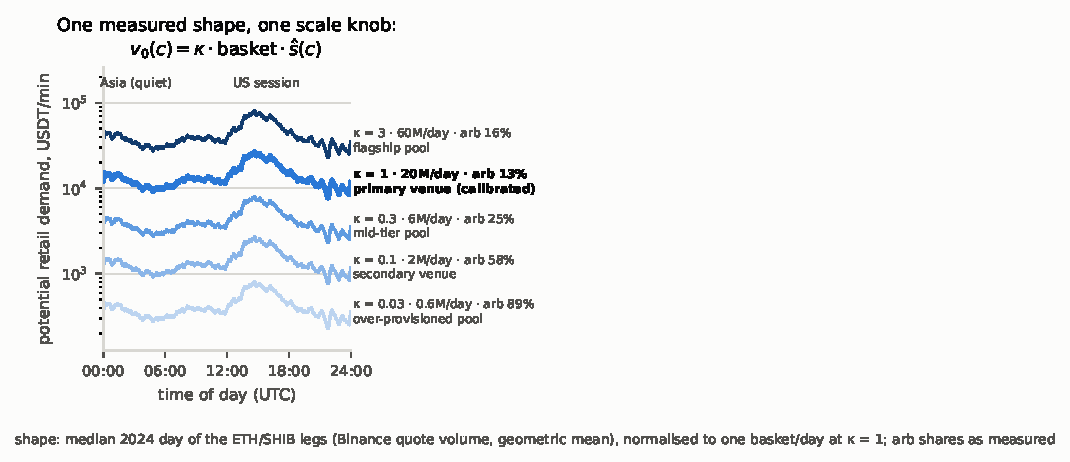
\includegraphics[width=\columnwidth]{Image/uu_demand_calibration.pdf}
  \caption{Demand calibration, Eq.~\eqref{eq:uu-demand}: the intraday
    shape $\hat{s}(c)$ is measured (median 2024 day of the pair's Binance
    legs); the single knob $\kappa$ scales its height, and the height
  sets the arbitrage share of volume the experiment measures.}
  \label{fig:demand}
\end{figure}

\begin{figure*}[t]
  \centering
  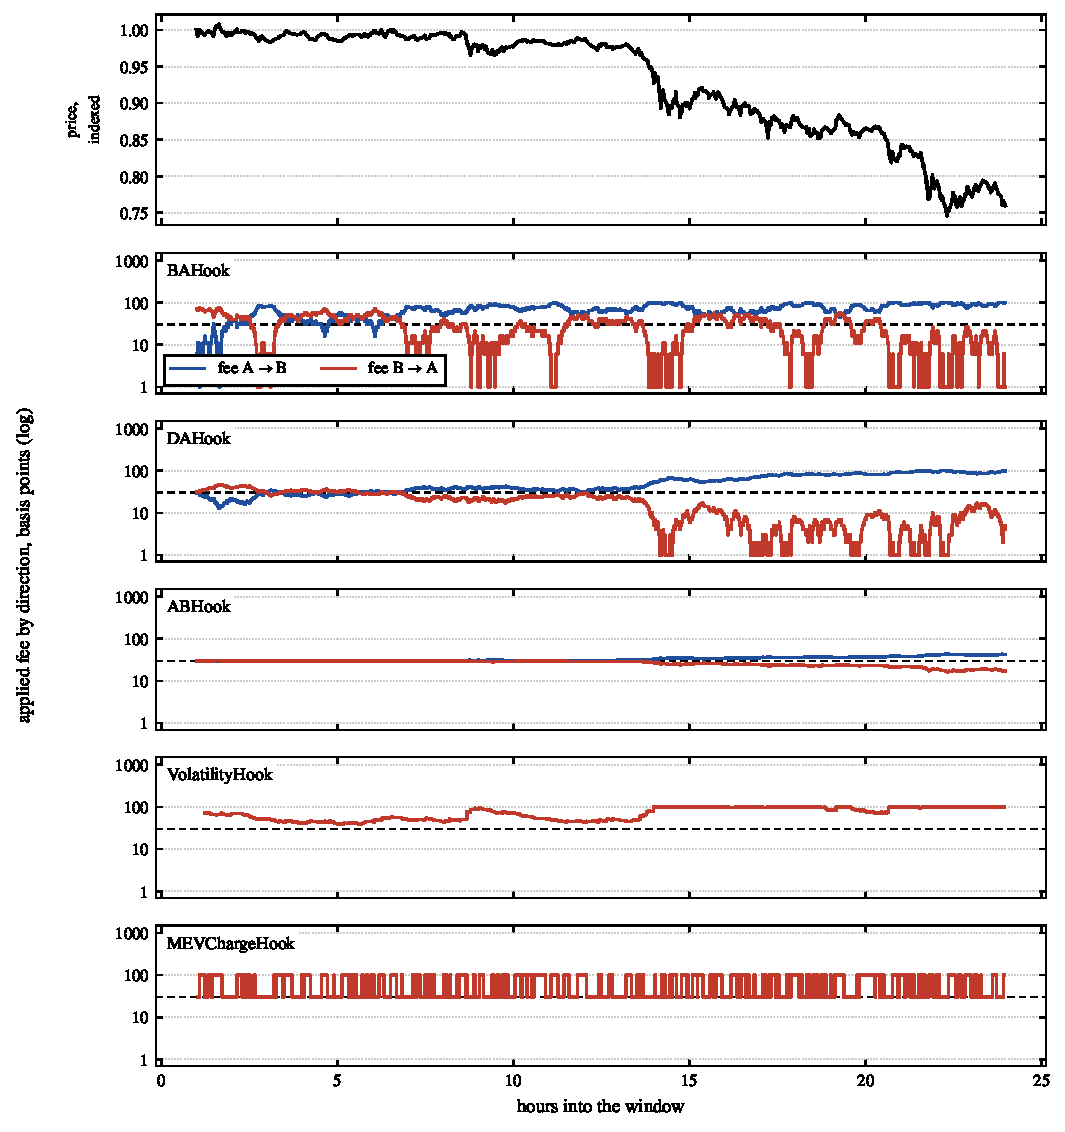
\includegraphics[width=.82\textwidth]{Image/uu_fee_response.pdf}
  \caption{What each hook actually charged through one high-volatility
    ETH/SHIB day (2024-03-01, 20~gwei, $\kappa{=}1$; log fee axis shared
    across panels; dashed = the 30~bps baseline). Each mark is the fee of
    an executed swap, held forward; for the directional hooks the two
    directions' fees interleave as swap direction alternates, which
  produces the sawtooth.}
  \label{fig:fee-response}
\end{figure*}

\subsection{Design and Statistics}

One operating point is a full factorial over 9 policy configurations
(five hook policies --- \texttt{BAHook}, \texttt{DAHook},
  \texttt{ABHook}, \texttt{MEVChargeHook}, and a volatility hook driven
  by an EMA of per-minute price variance --- and static baselines at
5/30/60/100~bps) $\times$ 3 pairs $\times$ 72 windows $\times$ 3 gas
scenarios --- 5{,}832 cells; five operating points give 29{,}160 cells.
Figure~\ref{fig:fee-response} illustrates the hooks' characters on one
stormy example day before any aggregation: the directional ratchets
split --- the side the market leaves gets dearer, the opposite one
cheaper --- the constant-sum hook barely re-aims its budget, the
volatility hook glides to the fee ceiling as variance arrives, and the
size-surcharge hook alternates between its base and capped rate.
The LP outcome of a cell is
$\mathrm{net} = R_f - IL = -L_{\mathrm{net}}$ of the main paper's
fee-adjusted loss, Eq.~(M4): the LP's
position and accrued fees against simply holding the deposit, all
marked at end-of-window prices.\footnote{The artifact additionally
  reports a trade-time valuation (each trade marked at the price of its
own moment); every finding below is unchanged under it.}

Every comparison is \emph{paired}: a policy's window result is
differenced against the pre-declared 30~bps static baseline on the same
window, pair, and gas price, removing the day-to-day variation that
dwarfs policy effects. Effects are reported as the median paired
difference with a 95\% percentile-bootstrap confidence interval
(10{,}000 seeded resamples); a comparison counts as a win or loss only
if the interval excludes zero. Headline
numbers aggregate cell-first (one median per pair$\times$regime$\times$gas
cell, then across cells), so three gas scenarios of one day are never
treated as independent observations.\footnote{The analysis CSVs also
  carry classical Wilcoxon signed-rank tests with Benjamini--Hochberg
  correction across the ${\sim}300$ comparisons; they agree with the
intervals in ${\sim}96\%$ of cases and are not used in the text.}
A post-hoc comparison against the best static fee in the box (60~bps) is
reported and labeled exploratory.

\subsection{Results}

\begin{table}[t]
  \caption{Median paired advantage over the 30~bps static baseline at
    the reference point ($\kappa{=}1$): median across the 18
    volatile-pair strata, 95\% bootstrap CI. Negative = worse than the
  baseline.}
  \label{tab:headline}
  \centering
  \footnotesize
  \begin{tabular}{lr}
    \toprule
    \textbf{Policy} & \textbf{advantage vs 30 bps, USDT/window}\\
    \midrule
    Static 60 bps         & $-2\;[-186,+266]$\\
    \texttt{BAHook}       & $-100\;[-453,+350]$\\
    \texttt{DAHook}       & $-235\;[-381,-104]$\\
    \texttt{ABHook}       & $-460\;[-630,-288]$\\
    Volatility hook       & $-752\;[-1069,-280]$\\
    \texttt{MEVChargeHook}& $-913\;[-1659,-728]$\\
    \bottomrule
  \end{tabular}
\end{table}

\subsubsection{No unconditional winner}
Table~\ref{tab:headline} gives the reference-point headline: no
evaluated dynamic policy beats the static 30~bps baseline; four lose
decisively and \texttt{BAHook} is indistinguishable from it. The
same holds at every other operating point --- pooled across regimes and
gas scenarios, no hook's interval clears zero at any $\kappa$
(Fig.~\ref{fig:kappa-trend-high}, companion pooled figure in the
artifact). The static fee curve itself has an interior optimum: mean
outcomes of $1.6$k$/11.9$k$/11.9$k$/7.9$k USDT per window at
5/30/60/100~bps, a 30--60~bps plateau consistent with the model's
$\arg\max_f f e^{-\lambda|r(f)|}\approx 2/\lambda\approx 43$~bps ---
with the caveat that this optimum's location follows from the assumed
participation function.

\subsubsection{A fee policy prices flow; it does not protect}
Decomposing the paired differences, the impermanent-loss term is
policy-invariant (single-digit USDT against fee-income effects in the
hundreds): arbitrage pins the end-of-window pool price to the external
price under every policy, so adaptation cannot reduce adverse selection
in this model --- it can only price the flow, and it prices it slightly
worse than a well-chosen constant while paying its own gas premium on
top.

\begin{figure}[t]
  \centering
  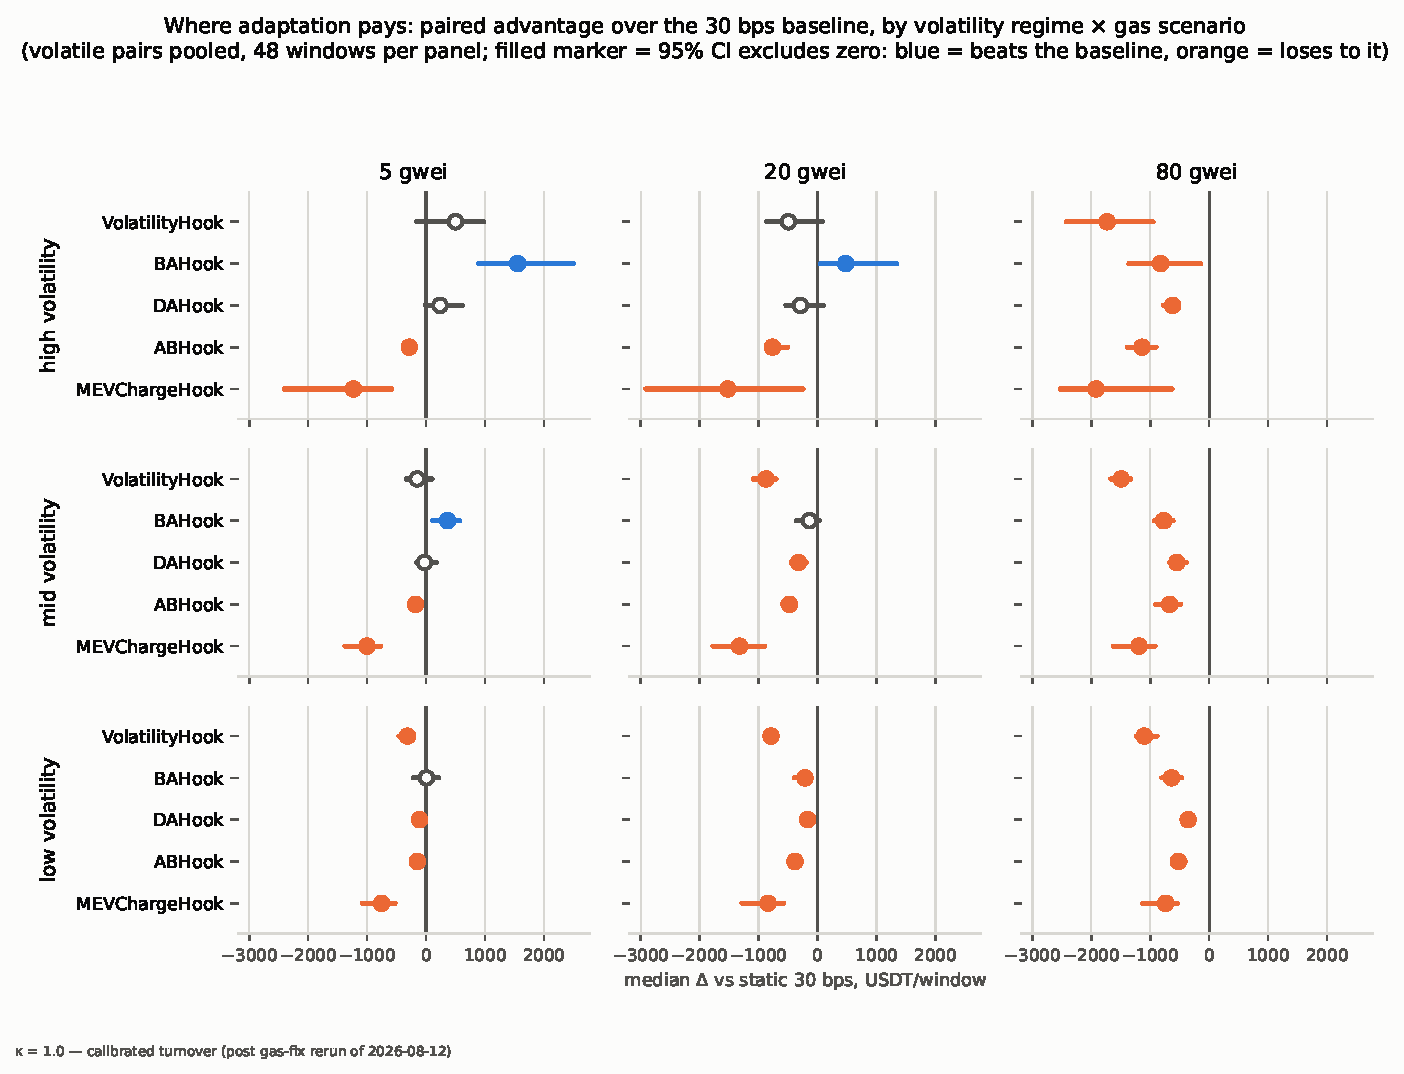
\includegraphics[width=\columnwidth]{Image/uu_regime_gas_grid.pdf}
  \caption{Conditional structure at $\kappa{=}1$: median paired
    advantage over the 30~bps baseline by volatility regime $\times$ gas
    scenario (volatile pairs pooled, 48 windows per panel; filled marker =
  95\% CI excludes zero; blue wins, orange loses).}
  \label{fig:grid}
\end{figure}

\begin{figure}[t]
  \centering
  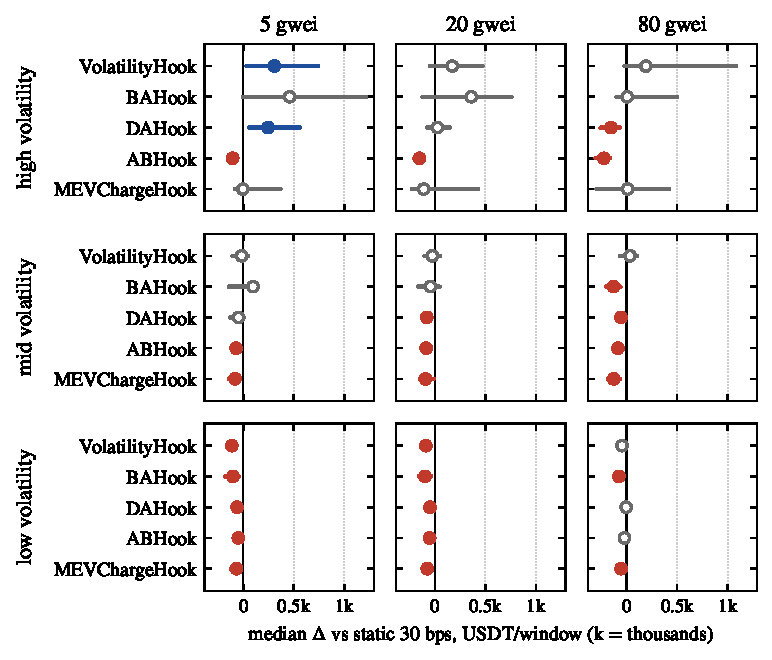
\includegraphics[width=\columnwidth]{Image/uu_t01_regime_gas_grid.pdf}
  \caption{The same decomposition at the informed-heavy point
    ($\kappa{=}0.1$, arbitrage 58\% of volume): the storm--cheap-gas
  corner strengthens and changes owners.}
  \label{fig:grid-t01}
\end{figure}

\begin{figure}[t]
  \centering
  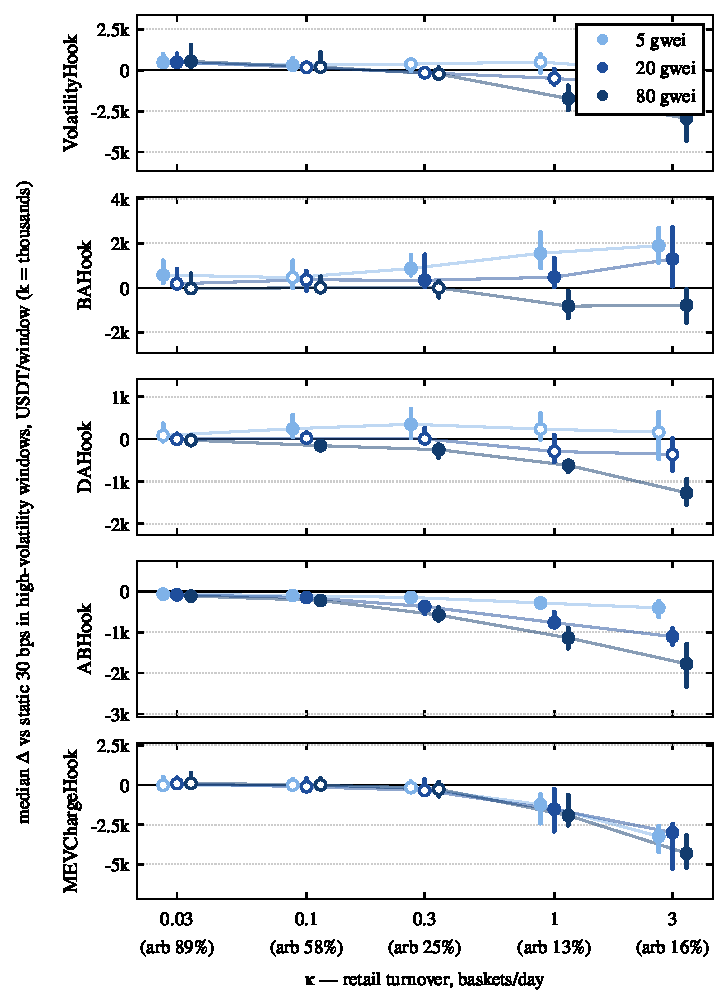
\includegraphics[width=\columnwidth]{Image/uu_kappa_trend_high.pdf}
  \caption{The storm slice across the retail scale: advantage over the
  baseline in high-volatility windows, by $\kappa$ and gas scenario.}
  \label{fig:kappa-trend-high}
\end{figure}

\subsubsection{Where adaptation does pay}
Crossing the two experimental axes reveals a robust conditional
structure (Fig.~\ref{fig:grid}). At $\kappa{=}1$, \texttt{BAHook} beats
the baseline in high-volatility windows at 5~gwei by
$+1{,}556\;[+894,+2{,}501]$ USDT per window and in mid-volatility
windows at 5~gwei by $+367\;[+115,+571]$;
at 80~gwei every policy loses or ties. The corner replicates at every
operating point with a clean hand-over of ownership
(Fig.~\ref{fig:kappa-trend-high}): at retail-dominated mixes
($\kappa\ge 0.3$) it belongs to \texttt{BAHook}; at informed-heavy mixes
($\kappa\le 0.1$) to the volatility hook and \texttt{DAHook}
($+308\;[+32,+742]$ and $+246\;[+59,+563]$ at $\kappa{=}0.1$,
Fig.~\ref{fig:grid-t01}); and at the
arbitrage-dominated extreme ($\kappa{=}0.03$) the volatility hook wins
storms at \emph{all three} gas prices --- the retail-gas channel is
irrelevant when there is hardly any retail. Read relatively (artifact
figures), every policy improves monotonically with volatility at every
gas level and degrades monotonically with gas in every regime.

\subsubsection{Gas is a first-order term}
The mechanism behind the gas gradient is the policies' own overhead:
oracle-reading hooks cost 108--124k gas per swap against the static
hook's 76k, retail prices that difference into
Eq.~\eqref{eq:uu-r}, and at 80~gwei even the static hook's
${\sim}\$19$ per swap is ${\sim}47$~bps of a typical \$4{,}000 retail
trade --- transaction costs rival the fee box itself. Consistently, the
informed share of volume rises with gas (12.4\% to 13.7\% across
5$\to$80~gwei at $\kappa{=}1$): small retail is priced out first.

\subsubsection{Summary}
None of the evaluated dynamic policies outperforms a well-chosen static
fee unconditionally. A reproducible conditional advantage exists in
high-volatility windows at low gas prices; which policy carries it
depends on the informed share of flow, and the advantage is consumed by
the policies' own gas premium as gas rises. The framework's contribution
is that this conditional structure is measurable at all --- paired,
reproducible, and decomposed along pre-declared axes.

\subsection{Threats to Validity}

The declared model limits: retail has no strategy and no correlated
demand; one arbitrageur acts once per candle with perfect information
and no mempool competition; liquidity is passive and full-range; mock
feeds validate integration, not live oracle behavior; the retail scale
$\kappa$ is an assumption swept over two orders of magnitude rather than
calibrated to real pools; retail lumpiness is fixed at one trade per
direction per minute; results cover one year, three pairs, one venue's
data, and a single RNG seed (a five-seed robustness appendix is defined
in the artifact). The conditional corner finding was not pre-registered
and is reported as observed structure; the unconditional findings and
the failed-and-reported gas prediction follow the pre-registered
protocol.

\appendices

\section{Evaluated Policies in Detail}
\label{app:policies}

All policies share the fee box $[1,100]$~bps (fees are \texttt{uint24}
values in hundredths of a basis point) and the same harness path;
``measured gas'' is the EVM-measured median per swap including the 21k
intrinsic transaction cost. Directional fees are written
$f^{0\to1}$ (selling token0) and $f^{1\to0}$; all start at 30~bps
unless noted.

\subsection{Static baselines (\texttt{MyHook})}
A constant fee $f\in\{5,30,60,100\}$~bps, identical in both directions,
never updated. Measured gas: 76--77k. These anchor every comparison:
30~bps is the pre-declared baseline, and the four levels trace the
static fee curve whose interior optimum the model predicts at
$2/\lambda$.

\subsection{\texttt{DAHook} --- deal-adaptive directional ratchet}
Endogenous (no oracle; its feed arguments are unused). After every
executed swap in direction $d$,
\begin{equation}
  f^{d}\leftarrow f^{d}+\delta,\qquad
  f^{-d}\leftarrow f^{-d}-\delta,\qquad \delta=1~\mathrm{bps},
  \label{eq:dahook}
\end{equation}
each side clamped to the box. The hook prices \emph{realized flow
direction}: sustained one-sided flow makes that direction progressively
dearer and the return path cheaper --- a micro market-maker skewing its
quotes. Update granularity: every trade. Measured gas: 88k (the
cheapest hook). In Fig.~\ref{fig:fee-response} its two series diverge
smoothly as the downtrend produces persistent directional flow.

\subsection{\texttt{BAHook} --- block-adaptive oracle ratchet}
Oracle-driven: two Chainlink-compatible feeds give the external ratio
$\rho_b=p_{0,b}/p_{1,b}$. At most once per block,
\begin{equation}
  f^{0\to1}\leftarrow f^{0\to1}+\delta\,\operatorname{sgn}(\rho_{b-1}-\rho_b),
  \qquad
  f^{1\to0}\leftarrow f^{1\to0}-\delta\,\operatorname{sgn}(\rho_{b-1}-\rho_b),
  \label{eq:bahook}
\end{equation}
with step $\delta=5$~bps, each side clamped to the box: when the
external price of token0 falls, selling token0 into the pool (the
direction an arbitrageur would trade) becomes dearer, and conversely.
A dealer widening the side the market is leaving. Update granularity:
block. Measured gas: 108k (two feed reads per update). This is the
policy that owns the storm corner at retail-heavy operating points.

\subsection{\texttt{ABHook} --- constant-sum reallocation}
Endogenous: it watches the \emph{pool's own} price, not a feed (its
feed arguments are unused). With $\Delta_t$ the relative change of the
pool's $\sqrt{\text{price}}$ since the previous swap,
\begin{equation}
  f^{0\to1}\leftarrow
  \operatorname{clamp}\!\left(f^{0\to1}-c\,\Delta_t\right),\qquad
  f^{1\to0}=K-f^{0\to1},
  \label{eq:abhook}
\end{equation}
with sensitivity $c=100$~bps per unit relative move and the invariant
$f^{0\to1}+f^{1\to0}=K=60$~bps at all times, which confines each side
to $[1,59]$~bps. The hook never changes its total fee \emph{budget} ---
it only re-aims it against the direction the pool price is moving, so
it is the cleanest test of whether reallocation alone pays (it does
not: it loses in every cell of every matrix). Update granularity: every
trade. Measured gas: 94k.

\subsection{Volatility hook --- symmetric level control}
Oracle-driven and symmetric. Per block it updates an exponentially
weighted per-minute variance of the external ratio's relative change
(weight $\alpha=0.1$, the squared move divided by the elapsed minutes),
and charges
\begin{equation}
  f=\operatorname{clamp}\!\left(f_{\mathrm{base}}
  +c\,\hat{\sigma}\right),\qquad
  f_{\mathrm{base}}=20~\mathrm{bps},\quad c=2\times10^{6},
  \label{eq:volhook}
\end{equation}
in both directions, where $\hat{\sigma}$ is the per-minute standard
deviation estimate. The constants map the measured 2024 minute-sigma
range onto the box: calm ($\hat\sigma\!\approx\!4\times10^{-4}$)
$\to$ ${\sim}28$~bps, stormy ($\hat\sigma\!\approx\!2\times10^{-3}$)
$\to$ ${\sim}60$~bps, extremes saturate at the ceiling. This is the
policy that owns the storm corner at informed-heavy operating points.
Measured gas: 123k (the dearest: two feed reads plus estimator state).

\subsection{\texttt{MEVChargeHook} --- size- and history-dependent charge}
Endogenous and symmetric in direction, but the only policy whose fee
depends on the \emph{trade} rather than the market: on top of a 30~bps
base it applies a time-decaying surcharge when the same sender has
recently traded (cooldown 15~s) and a surcharge increasing in trade
size, capped at the box ceiling --- so its effective range is
$[30,100]$~bps. Because the fee reads the trade size, the arbitrageur's
closed form does not apply and its optimal trade is found by ternary
search. Measured gas: 95k. In Fig.~\ref{fig:fee-response} it alternates
between base and cap as the surcharge triggers fire.

\section{Derivation of the Arbitrage Optimum}
\label{app:arb}

Within one tick range a Uniswap v3/v4 pool with liquidity $L$ obeys the
constant-product amount relations in sqrt-price coordinates: moving the
pool price from $\sqrt{p}=s_1$ to $s_2$ exchanges
\begin{equation}
  \Delta y = L\,(s_2-s_1),\qquad
  \Delta x = L\left(\frac{1}{s_1}-\frac{1}{s_2}\right),
  \label{eq:app-amounts}
\end{equation}
and the LP fee $f$ ($\gamma=1-f$) is charged on the input amount before
it enters the curve.

\subsubsection{Band edges}
Selling token0 (zero-for-one) at pool sqrt-price $s$ realizes a marginal
price $\gamma s^{2}$ in token1 per token0; the trade is profitable
against the external price $P$ while $\gamma s^{2}>P$, i.e. while
$s>\sqrt{P/\gamma}=t_{0\to1}$. Buying token0 costs $s^{2}/\gamma$
marginally and is profitable while $s^{2}/\gamma<P$, i.e. while
$s<\sqrt{P\gamma}=t_{1\to0}$. Hence the no-arbitrage band
$[P\gamma,\,P/\gamma]$ on the pool price, and the profit-maximizing
trade stops exactly at the near edge: the integrand of marginal profit
changes sign there, so profit is unimodal in trade size with its
maximum at the edge.

\subsubsection{Sell side}
Moving the pool from $s$ down to $t=t_{0\to1}$ requires a net token0
input $\Delta x=L(1/t-1/s)$, for which the trader pays the grossed-up
$\Delta x/\gamma$, and yields $\Delta y=L(s-t)$ of token1. Valued at the
external price $P=\gamma t^{2}$,
\begin{align}
  \Pi_{0\to1}
  &= L(s-t)-\frac{P}{\gamma}\,L\!\left(\frac{1}{t}-\frac{1}{s}\right)
  = L(s-t)-L\,t^{2}\,\frac{s-t}{ts}\nonumber\\
  &= L(s-t)\!\left(1-\frac{t}{s}\right)
  = \frac{L\,(s-t)^{2}}{s}.
  \label{eq:app-sell}
\end{align}

\subsubsection{Buy side}
Moving the pool from $s$ up to $t=t_{1\to0}$ requires net token1 input
$L(t-s)$, paid as $L(t-s)/\gamma$, and yields
$\Delta x=L(1/s-1/t)$ of token0 worth $P\,\Delta x$. With
$P=t^{2}/\gamma$,
\begin{align}
  \Pi_{1\to0}
  &= \frac{t^{2}}{\gamma}\,L\,\frac{t-s}{ts}-\frac{L(t-s)}{\gamma}
  = \frac{L(t-s)}{\gamma}\!\left(\frac{t}{s}-1\right)\nonumber\\
  &= \frac{L\,(t-s)^{2}}{\gamma\,s}.
  \label{eq:app-buy}
\end{align}
The extra $1/\gamma$ relative to Eq.~\eqref{eq:app-sell} arises because
the fee is charged in token1 --- the numeraire the profit is measured in
--- so, unlike the sell side, it does not cancel against the external
valuation of the input.

\subsubsection{Gas}
Gas adds a size-independent cost $g\,p_{\mathrm{gas}}$, which shifts the
profit curve down without moving its maximum; checking
$\Pi^{*}>g\,p_{\mathrm{gas}}$ after the size optimization is therefore
equivalent to including gas inside it (the arbitrageur cannot split a
trade across transactions in this model). For a size-dependent fee the
closed form is replaced by a ternary search, valid because an input fee
non-decreasing in size preserves unimodality.

\IfFileExists{IEEEtran.bst}{\bibliographystyle{IEEEtran}}{\bibliographystyle{unsrt}}
\bibliography{reference}

\end{document}
